% Options for packages loaded elsewhere
\PassOptionsToPackage{unicode}{hyperref}
\PassOptionsToPackage{hyphens}{url}
%
\documentclass[
  man]{apa7}
\usepackage{amsmath,amssymb}
\usepackage{iftex}
\ifPDFTeX
  \usepackage[T1]{fontenc}
  \usepackage[utf8]{inputenc}
  \usepackage{textcomp} % provide euro and other symbols
\else % if luatex or xetex
  \usepackage{unicode-math} % this also loads fontspec
  \defaultfontfeatures{Scale=MatchLowercase}
  \defaultfontfeatures[\rmfamily]{Ligatures=TeX,Scale=1}
\fi
\usepackage{lmodern}
\ifPDFTeX\else
  % xetex/luatex font selection
\fi
% Use upquote if available, for straight quotes in verbatim environments
\IfFileExists{upquote.sty}{\usepackage{upquote}}{}
\IfFileExists{microtype.sty}{% use microtype if available
  \usepackage[]{microtype}
  \UseMicrotypeSet[protrusion]{basicmath} % disable protrusion for tt fonts
}{}
\makeatletter
\@ifundefined{KOMAClassName}{% if non-KOMA class
  \IfFileExists{parskip.sty}{%
    \usepackage{parskip}
  }{% else
    \setlength{\parindent}{0pt}
    \setlength{\parskip}{6pt plus 2pt minus 1pt}}
}{% if KOMA class
  \KOMAoptions{parskip=half}}
\makeatother
\usepackage{xcolor}
\usepackage{graphicx}
\makeatletter
\newsavebox\pandoc@box
\newcommand*\pandocbounded[1]{% scales image to fit in text height/width
  \sbox\pandoc@box{#1}%
  \Gscale@div\@tempa{\textheight}{\dimexpr\ht\pandoc@box+\dp\pandoc@box\relax}%
  \Gscale@div\@tempb{\linewidth}{\wd\pandoc@box}%
  \ifdim\@tempb\p@<\@tempa\p@\let\@tempa\@tempb\fi% select the smaller of both
  \ifdim\@tempa\p@<\p@\scalebox{\@tempa}{\usebox\pandoc@box}%
  \else\usebox{\pandoc@box}%
  \fi%
}
% Set default figure placement to htbp
\def\fps@figure{htbp}
\makeatother
\setlength{\emergencystretch}{3em} % prevent overfull lines
\providecommand{\tightlist}{%
  \setlength{\itemsep}{0pt}\setlength{\parskip}{0pt}}
\setcounter{secnumdepth}{-\maxdimen} % remove section numbering
% Make \paragraph and \subparagraph free-standing
\makeatletter
\ifx\paragraph\undefined\else
  \let\oldparagraph\paragraph
  \renewcommand{\paragraph}{
    \@ifstar
      \xxxParagraphStar
      \xxxParagraphNoStar
  }
  \newcommand{\xxxParagraphStar}[1]{\oldparagraph*{#1}\mbox{}}
  \newcommand{\xxxParagraphNoStar}[1]{\oldparagraph{#1}\mbox{}}
\fi
\ifx\subparagraph\undefined\else
  \let\oldsubparagraph\subparagraph
  \renewcommand{\subparagraph}{
    \@ifstar
      \xxxSubParagraphStar
      \xxxSubParagraphNoStar
  }
  \newcommand{\xxxSubParagraphStar}[1]{\oldsubparagraph*{#1}\mbox{}}
  \newcommand{\xxxSubParagraphNoStar}[1]{\oldsubparagraph{#1}\mbox{}}
\fi
\makeatother
% definitions for citeproc citations
\NewDocumentCommand\citeproctext{}{}
\NewDocumentCommand\citeproc{mm}{%
  \begingroup\def\citeproctext{#2}\cite{#1}\endgroup}
\makeatletter
 % allow citations to break across lines
 \let\@cite@ofmt\@firstofone
 % avoid brackets around text for \cite:
 \def\@biblabel#1{}
 \def\@cite#1#2{{#1\if@tempswa , #2\fi}}
\makeatother
\newlength{\cslhangindent}
\setlength{\cslhangindent}{1.5em}
\newlength{\csllabelwidth}
\setlength{\csllabelwidth}{3em}
\newenvironment{CSLReferences}[2] % #1 hanging-indent, #2 entry-spacing
 {\begin{list}{}{%
  \setlength{\itemindent}{0pt}
  \setlength{\leftmargin}{0pt}
  \setlength{\parsep}{0pt}
  % turn on hanging indent if param 1 is 1
  \ifodd #1
   \setlength{\leftmargin}{\cslhangindent}
   \setlength{\itemindent}{-1\cslhangindent}
  \fi
  % set entry spacing
  \setlength{\itemsep}{#2\baselineskip}}}
 {\end{list}}
\usepackage{calc}
\newcommand{\CSLBlock}[1]{\hfill\break\parbox[t]{\linewidth}{\strut\ignorespaces#1\strut}}
\newcommand{\CSLLeftMargin}[1]{\parbox[t]{\csllabelwidth}{\strut#1\strut}}
\newcommand{\CSLRightInline}[1]{\parbox[t]{\linewidth - \csllabelwidth}{\strut#1\strut}}
\newcommand{\CSLIndent}[1]{\hspace{\cslhangindent}#1}
\ifLuaTeX
\usepackage[bidi=basic]{babel}
\else
\usepackage[bidi=default]{babel}
\fi
\babelprovide[main,import]{english}
% get rid of language-specific shorthands (see #6817):
\let\LanguageShortHands\languageshorthands
\def\languageshorthands#1{}
\ifLuaTeX
  \usepackage[english]{selnolig} % disable illegal ligatures
\fi
% Manuscript styling
\usepackage{upgreek}
\captionsetup{font=singlespacing,justification=justified}

% Table formatting
\usepackage{longtable}
\usepackage{lscape}
% \usepackage[counterclockwise]{rotating}   % Landscape page setup for large tables
\usepackage{multirow}		% Table styling
\usepackage{tabularx}		% Control Column width
\usepackage[flushleft]{threeparttable}	% Allows for three part tables with a specified notes section
\usepackage{threeparttablex}            % Lets threeparttable work with longtable

% Create new environments so endfloat can handle them
% \newenvironment{ltable}
%   {\begin{landscape}\centering\begin{threeparttable}}
%   {\end{threeparttable}\end{landscape}}
\newenvironment{lltable}{\begin{landscape}\centering\begin{ThreePartTable}}{\end{ThreePartTable}\end{landscape}}

% Enables adjusting longtable caption width to table width
% Solution found at http://golatex.de/longtable-mit-caption-so-breit-wie-die-tabelle-t15767.html
\makeatletter
\newcommand\LastLTentrywidth{1em}
\newlength\longtablewidth
\setlength{\longtablewidth}{1in}
\newcommand{\getlongtablewidth}{\begingroup \ifcsname LT@\roman{LT@tables}\endcsname \global\longtablewidth=0pt \renewcommand{\LT@entry}[2]{\global\advance\longtablewidth by ##2\relax\gdef\LastLTentrywidth{##2}}\@nameuse{LT@\roman{LT@tables}} \fi \endgroup}

% \setlength{\parindent}{0.5in}
% \setlength{\parskip}{0pt plus 0pt minus 0pt}

% Overwrite redefinition of paragraph and subparagraph by the default LaTeX template
% See https://github.com/crsh/papaja/issues/292
\makeatletter
\renewcommand{\paragraph}{\@startsection{paragraph}{4}{\parindent}%
  {0\baselineskip \@plus 0.2ex \@minus 0.2ex}%
  {-1em}%
  {\normalfont\normalsize\bfseries\itshape\typesectitle}}

\renewcommand{\subparagraph}[1]{\@startsection{subparagraph}{5}{1em}%
  {0\baselineskip \@plus 0.2ex \@minus 0.2ex}%
  {-\z@\relax}%
  {\normalfont\normalsize\itshape\hspace{\parindent}{#1}\textit{\addperi}}{\relax}}
\makeatother

\makeatletter
\usepackage{etoolbox}
\patchcmd{\maketitle}
  {\section{\normalfont\normalsize\abstractname}}
  {\section*{\normalfont\normalsize\abstractname}}
  {}{\typeout{Failed to patch abstract.}}
\patchcmd{\maketitle}
  {\section{\protect\normalfont{\@title}}}
  {\section*{\protect\normalfont{\@title}}}
  {}{\typeout{Failed to patch title.}}
\makeatother

\usepackage{xpatch}
\makeatletter
\xapptocmd\appendix
  {\xapptocmd\section
    {\addcontentsline{toc}{section}{\appendixname\ifoneappendix\else~\theappendix\fi\\: #1}}
    {}{\InnerPatchFailed}%
  }
{}{\PatchFailed}
\keywords{reliability, teaching effectiveness, fairness, grading, evaluations}
\DeclareDelayedFloatFlavor{ThreePartTable}{table}
\DeclareDelayedFloatFlavor{lltable}{table}
\DeclareDelayedFloatFlavor*{longtable}{table}
\makeatletter
\renewcommand{\efloat@iwrite}[1]{\immediate\expandafter\protected@write\csname efloat@post#1\endcsname{}}
\makeatother
\usepackage{lineno}

\linenumbers
\usepackage{csquotes}
\makeatletter
\renewcommand{\paragraph}{\@startsection{paragraph}{4}{\parindent}%
  {0\baselineskip \@plus 0.2ex \@minus 0.2ex}%
  {-1em}%
  {\normalfont\normalsize\bfseries\typesectitle}}

\renewcommand{\subparagraph}[1]{\@startsection{subparagraph}{5}{1em}%
  {0\baselineskip \@plus 0.2ex \@minus 0.2ex}%
  {-\z@\relax}%
  {\normalfont\normalsize\bfseries\itshape\hspace{\parindent}{#1}\textit{\addperi}}{\relax}}
\makeatother

\usepackage{bookmark}
\IfFileExists{xurl.sty}{\usepackage{xurl}}{} % add URL line breaks if available
\urlstyle{same}
\hypersetup{
  pdftitle={The Reliability of Student Evaluations of Teaching},
  pdfauthor={Erin M. Buchanan1, Jacob Miranda2, \& Christian Stephens2},
  pdflang={en-EN},
  pdfkeywords={reliability, teaching effectiveness, fairness, grading, evaluations},
  hidelinks,
  pdfcreator={LaTeX via pandoc}}

\title{The Reliability of Student Evaluations of Teaching}
\author{Erin M. Buchanan\textsuperscript{1}, Jacob Miranda\textsuperscript{2}, \& Christian Stephens\textsuperscript{2}}
\date{}


\shorttitle{RELIABILITY EVALUATIONS}

\authornote{

The authors made the following contributions. Erin M. Buchanan: Conceptualization, Writing - Original Draft Preparation, Writing - Review \& Editing, Analysis; Jacob Miranda: Writing - Original Draft Preparation; Christian Stephens: Writing - Original Draft Preparation.

Correspondence concerning this article should be addressed to Erin M. Buchanan, 326 Market St., Harrisburg, PA 17010. E-mail: \href{mailto:ebuchanan@harrisburgu.edu}{\nolinkurl{ebuchanan@harrisburgu.edu}}

}

\affiliation{\vspace{0.5cm}\textsuperscript{1} Harrisburg University of Science and Technology\\\textsuperscript{2} University of Alabama}

\abstract{%
Student evaluations of teaching are regularly used within college classrooms to gauge effectiveness of instruction, provide evidence for administrative decision making, and inform instructors of course feedback. Teaching evaluations are thought to be a reliable measure, but few studies have explored their reliability over time. We investigated over 30 years of teaching evaluations to determine the reliability of teaching evaluations across course, instructor, and time. We used these estimates to determine the stability of reliability estimates over time and tried to predict reliability using student ratings of instructor fairness. Instructors teaching the same course multiple times within the same semester showed the highest reliability estimates. The reliability of instructor's evaluations showed a small decrease over time. Evaluations should be carefully considered given the context of the semester received and potentially paired with other measures of teaching effectiveness.
}



\begin{document}
\maketitle

In the United States, college and university professors are
evaluated to varying degrees on research productivity, service, and
teaching effectiveness. These dimensions are often used for high-stakes
administration decisions, including hiring, retention, promotion, pay,
and tenure (Freishtat, 2014; Hornstein, 2017; Spooren et al., 2013; Stroebe, 2020).
Depending on the institution, a major failure of one of these evaluative
dimensions could jeopardize a professor's position within the
department; thus, professors are urged to maintain high standards of
research, service, and teaching. Indeed, the vast majority of the 9,000
professors polled by the \emph{American Association of University Professors}
believed the teaching evaluative dimension should be taken as seriously
as research and service (Flaherty, 2015). The consequences of teacher
effectiveness may motivate collegiate faculty into actively considering
the quality of their classroom.

Teaching effectiveness can be defined as the degree to which student
achievement is facilitated (i.e., how much have students learned in a
particular course, P. A. Cohen, 1981). Generally, assessments of teaching
effectiveness come from student evaluations of teaching (SETs) or the
course itself (e.g., ``Student Opinion of Instruction,'' ``Students Opinion
of Teaching Effectiveness,'' ``Students Evaluation of Faculty,'' ``Overall
Course Ratings,'' ``Instruction Rating,'' P. A. Cohen, 1981; Flaherty, 2020). Often
these metrics are described as evaluating the quality of the individual
or course (Gillmore et al., 1978; Marsh, 2007) by gauging multiple facets of teaching, such as an instructor's proficiency in communication, organization, presentation, and grading (Hattie \& Marsh, 1996).

Given the use of SETs in administrative decisions, both the reliability and validity of these measures should be demonstrated to ensure their utility. Instructors, in particular, have both a vested interest and skill set to evaluate the quality of measurement. If these evaluations are used to make high-stakes decisions that will alter a professors' career and standing within the workplace, it is important to be skeptical and scrutinize the decision metrics used. We are not the first to explore if SETs are reliable and valid measures of teaching effectiveness, but our approach makes a unique contribution by analyzing over 30 years of SET data to address this question in a more compelling way.

\subsection{Reliability}\label{reliability}

Past investigations of SETs concluded they are reliable measures
(Arubayi, 1987; Marsh \& Roche, 1997). Contemporary reviews have explored the
reliability of SETs when controlling for various factors. For example,
Benton and Cashin (2014) found SETs collected from the same class to be internally
consistent when teaching effectiveness was assessed through several
items. Even so, other data suggest that instructor, course, and student
factors each contribute meaningfully to the variance of student
evaluation ratings, which can influence their reliability
(Feistauer \& Richter, 2017). This result suggests SET ratings may be reliable over
time if the aspects of a classroom remain constant. However, few data
have explored the interactions of time with validity variables or how it
affects reliability among SETs in relation to perceived fairness
specifically. Little research investigating the reliability of SETs has
collected evaluations beyond two time points (e.g., two semesters or
less). There are some notable exceptions of longer periods of data being
collected for SETs in Boring et al. (2016), Marsh (2007), and Fan et al. (2019) and, our study extends this work by examining the reliability patterns of 30 years of SET data with respect to various moderating influences that may affect both reliability and validity of SETs.

\subsection{Validity}\label{validity}

Sheehan's (1975) review of instructor evaluation literature found such measures contained multiple potentially biasing factors. These include (1) student demographics: gender, class, age,
previous achievement, (2) class type: subject matter, size, degree
requirements, and (3) instructor qualities: gender, rank, gender-match to
student, etc. Decades later, studies still show that sexism
(MacNell et al., 2015; Mitchell \& Martin, 2018), racism (Smith \& Hawkins, 2011), and biases in general
pervade students' evaluations today in both traditional courses and
possibly online ones as well (Heffernan, 2022; O'Sullivan et al., 2014; Rovai et al., 2006; Zheng et al., 2023). Individual factors may also yield some influence on SET
ratings, including instructors' cultural background (Fan et al., 2019),
attractiveness (Felton et al., 2008; Wright, 2000), position ranking
(Johnson et al., 2013), and students' expected grade from the course (Chen et al., 2017; Crumbley et al., 2001; Marks, 2000). Biasing factors may even include the volume
of the instructor's voice and how legible their instructor's writing is
(W. E. Becker et al., 2012). Concerningly, Stroebe (2020) highlighted the danger of an incentive system tied to student ratings; specifically, instructors may be incentivized to be a less effective teacher (e.g., grade leniently, choose to teach courses based on student interest, etc.) rather than challenge students critically to boost their SET ratings.

Concerns of bias raised decades ago have not dissipated over time (Boring et al., 2016; Dunn et al., 2014; Hornstein, 2017; Uttl et al., 2017). Recent meta-analyses suggest SETs may be
entirely unrelated to material learned (Uttl et al., 2017), and potentially
biasing aspects cannot be altered due to their complex interactions
(Boring et al., 2016). While students' ratings may show some utility in
indicating to their peers which classes to pursue and which professor to
take (Stankiewicz, 2015), this usefulness may come at the cost of the professor's
self-efficacy (Boswell, 2016). While SETs are conceptually valuable
towards gaining insight on teacher effectiveness or course quality, the
many outstanding issues suggest they may not be valid measures. Even so,
some researchers argue that the complete removal of SETs from
administrative consideration is the wrong course of action
(Benton \& Ryalls, 2016). A more appropriate solution may be to utilize multiple
measures of teaching effectiveness simultaneously (eclass observation by
another instructor of the same material, peer reviews of course curriculum Benton \& Young, 2018; Berk, 2018; Esarey \& Valdes, 2020; Kornell \& Hausman, 2016). However, the cost of implementing
a more accurate, multi-pronged approach may be unrealistic given a
university's budget and expectations of the instructor. Instead, we may be able to potentially control for some biasing or moderating factors with additional items on the SET questionnaire, and our study explores the aspect of perceived fairness in grading.

\subsection{Perceived Fairness}\label{perceived-fairness}

Extant research broadly supports that SETs are influenced by students grades. Intriguingly as pointed out by Wright (2000), students' expectations of their final grades may not affect their SET ratings nearly as much as their perceived fairness of their grades or the grading process that produced them. For this reason, some instructors may feel pressured into reducing the rigor of their course for the sake of attaining higher SET ratings (Greenwald \& Gillmore, 1997; Marks, 2000). However, professors who are consistent, accurate, unbiased, and correctable in their grading may receive high SET ratings regardless of how much a student learns or what his/her final grade turns out to be (Horan et al., 2010; Leventhal, 1980). Students' grades may predict their SETs only so much as students perceive the grading processes as fair (Tata, 1999).

Students' perceptions of fairness may be more akin to comprehensive assessments of the instructor rather than face-value judgments of their expected grade. Perceived fairness may also play a multifactorial role in its influence on SETs. Tripp et al. (2019) found that students' perceived fairness of their instructors' grading processes affected their perceived fairness of their assigned grade, which then related to instructors' SETs. Additionally, \emph{perceived fairness of the course} workload and difficulty may be inversely related to \emph{perceived fairness of the grading process} as a challenging professor may be thought of as less fair (Marks, 2000). Access to grading criteria, frequency of feedback, and proactive instruction are other aspects of grading thought to explicitly affect perceived fairness (Pepper \& Pathak, 2008). Therefore, the perceived fairness of those aspects must also be considered when determining the impact of perceived fairness on SET ratings, especially when different professors teach the same course or teach multiple courses in the same semester. The validity and reliability of SETs may then partially hinge on the consistency of students' perceptions of fairness.

\subsection{The Current Study}\label{the-current-study}

The current study is similar in scope to recent work (Boring et al., 2016; Fan et al., 2019) in its analysis of teacher evaluations collected over an
extensive period. Boring et al. (2016)`s investigation on both French instructors
and U.S. teaching assistants' gender ranged across five years.
Similarly, Fan et al. (2019)`s investigated the topic across seven years. Their
utilization of multi-sections has been described as the gold standard
for researching students' ratings. However, it is important to continue
to assess the reliability and usefulness of SETs as the types of
students, student expectations, teaching pedagogy, grading practices,
and university administrative decisions change and evolve over time.

We believe the current study contributes to the literature in several
ways. When compared to the next largest study on SETs (Fan et al., 2019),we collected and analyzed three decades worth of data between 1987 and 2018 within an American population (vs seven years from 2010 - 2016 from an Australian population). Our dataset is publicly available online following best open science practices (Wilkinson et al., 2016). We believe this openness will provide value to educators
overall, and SET researchers specifically, by allowing future analyses to
explore the richness of this extensive dataset.

We aimed to analyze the reliability of students' ratings provided the \emph{same} or \emph{different} (i) instructor, (ii) course type, and/or (iii) semester of enrollment. This separation is paired with testing reliability over more than 30 years of data, extending previous work into new areas. We examined the impact of a potential validity variable on the reliability of ratings using perceived fairness of grading.Therefore, we sought to explore the
following research questions:

\begin{enumerate}
\def\labelenumi{\arabic{enumi})}
\tightlist
\item
  What is the reliability of student evaluations?
\item
  Are student evaluations reliable across time?
\item
  Is the average level of perceived fairness of the grading in the
  course a moderator of reliability in student evaluations over time?
\item
  Does the average variability in instructor fairness rating moderate
  reliability of student evaluations over time?
\end{enumerate}

The following was pre-registered as a secondary data analysis at:
\url{https://osf.io/czb4f}. The manuscript, code, and data can be found on
our Open Science Framework page at: \url{https://osf.io/k7zh2/} or GitHub:
\url{https://github.com/doomlab/Grade-Lean}. This manuscript was written
with the \emph{R} packages \emph{papaja} (Aust et al., 2022), \emph{rio} (J. Becker et al., 2021), \emph{dplyr}
(Wickham et al., 2020), \emph{nlme} (Pinheiro et al., 2017), \emph{ggplot2} (Wickham, 2016), \emph{MuMIn}
(Bartoń, 2020), \emph{ppcor} (Kim, 2015), and \emph{effectsize} (Ben-Shachar et al., 2020).

\section{Method}\label{method}

\subsection{Data Source}\label{data-source}

The archival study was conducted using data from the psychology
department at a large Midwestern public university. We used data from
2898
undergraduate, 274
mixed-level undergraduate, and
42 graduate
psychology classes taught from 1987 to 2018 that were evaluated by
students using the same 15-item instrument. Faculty followed set
procedures in distributing scan forms no more than two weeks before the
conclusion of the semester. A student was assigned to collect the forms
and deliver them to the departmental secretary. The instructor was
required to leave the room while students completed the forms. In the
last several years of evaluations, online versions of these forms were
used with faculty encouraged to give students time to complete them in
class while they were outside the classroom. The average sample size
before moving online was 25.13 (\emph{SD} = 25.45) students, while the
average sample size after moving online was 15.17 (\emph{SD} = 25.51).\footnote{Only
  a few semesters of online evaluation data are present in this dataset.}
Courses generally ranged from 10 to 30 for undergraduate courses with
the exception of introduction to psychology which was converted into a
large scale 300-person format. Graduate courses enrollment depended on
the size of the program but was generally 5 to 10 students.

\subsubsection{SET Questionnaire}\label{set-questionnaire}

The questionnaire given to students can be found at
\url{https://osf.io/4sphx}. These items were presented with a five-point
scale from 1 (\emph{strongly disagree}) to 5 (\emph{strongly agree}). The ratings were averaged for each course across students, and the sample size for each rating was included.

\subsubsection{Reliability}\label{reliability-1}

The specific formula for reliability is described in planned analysis. The reliability scores were generally created by comparing the overall instructor evaluation question: ``The overall quality of this course was among the top 20\% of those I have taken.'' of each instructor to every other instructor, controlling for sample size of the ratings. The pairwise combination of instructors in the dataset allowed us to create reliability scores for the same or different combinations of instructor, course, and semester of enrollment. These values were created in Research Question 1 and used for the rest of the analyses.

\subsubsection{Fairness}\label{fairness}

We used the question of ``The instructor used fair and appropriate methods in the determination of grades.'' The average rating of fairness for each course was calculated, as well as the standard deviation of fairness to examine variability in perceptions of fairness (i.e., large standard deviations mean that students disagree on fairness, while smaller values indicate more agreement).

\subsection{Planned Analyses}\label{planned-analyses}

The evaluations were filtered for those with at least fifteen student
ratings for the course (Rantanen, 2012). We performed a robustness check
for the first research question by running the same analyses again to
ensure the results were the same for different sample sizes. We used the
data when the sample size was at least \emph{n} = 10 up to \emph{n} = 14 (i.e., on
all evaluations with at least 10 ratings, then at least 11 ratings,
etc.) to determine if the reliability estimates are stable at lower
sample sizes. We first screened the dataset (two evaluation questions,
sample size for course) for accuracy errors (obvious typos in the data),
linearity (a linear relationship of the variables), normality (normal
distributions for the errors), and homoscedasticity (an even spread of
errors for the criterion variable at all parts of the independent
variable). The data were assumed to not have traditional ``outliers'', as
these evaluations represent true averages from student evaluations. If
the linearity assumption failed, we considered potential nonparametric
models to address non-linearity. Deviations from normality were noted
but the large sample size should provide robustness for any violations
of normality. If the errors appeared to be heteroscedastic, we used
bootstrapping to provide estimates and confidence intervals.

\begin{figure}
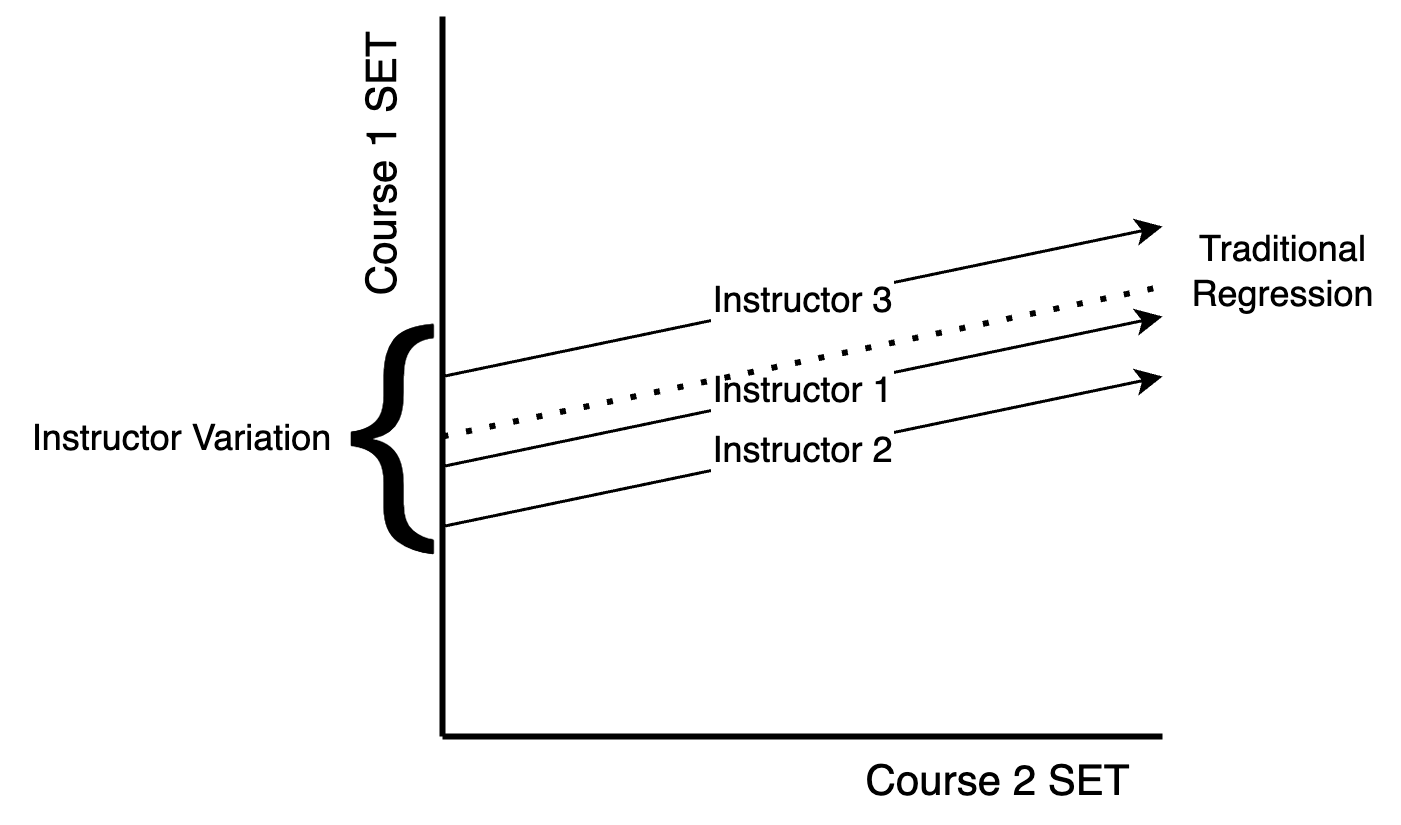
\includegraphics[width=4.67in]{includes/random_intercept} \caption{An example of Research Question 1 including random intercepts for instructor. Each instructor shows a different overall course average score where the regression line crosses the y-intercept. The traditional regression analysis (the dotted line) ignores differences in instructor by averaging over instructor.}\label{fig:figure-random-explain}
\end{figure}

This data was considered structured by instructor, meaning that each
instructor had multiple courses across multiple years (i.e., repeated
measures data); therefore, all analyses below were coded in \emph{R} using
the \emph{nlme} package (Pinheiro et al., 2017) to control for correlated error of
instructor as a random intercept in a multilevel model. Multilevel
models allow for analysis of repeated measures data without collapsing
by participant (i.e., each instructor/semester/course combination can be
kept separate without averaging over these measurements, Gelman, 2006).
Random intercept models are regression models on repeated data that
structure the data by a specified variable, which was instructor in this
analysis. Therefore, each instructor's overall average rating score was
allowed to vary within the analysis, as ratings would be expected to differ from instructor to instructor. In traditional regression
models, the intercept represents the grand mean of all of the data,
which would ignore differences in instructor. By including this
intercept, we were able to allow the intercept to vary by instructor,
and then measure the impact of the independent variables on the ratings
or reliability. Figure \ref{fig:figure-random-explain} this analysis might look visually for research question 1. In each of
the analyses described below, the number of students providing ratings
for the course was included as a control variable to even out
differences in course size as an influence in the results. This variable
was planned to be excluded if the models did not converge (i.e., did not
mathematically find an answer). The criterion variable and predictors
varied based on the research question, and these are described with each
analysis below.

\subsubsection{Research Question 1}\label{research-question-1}

In this research question, we examined the reliability of student
evaluations on the overall rating and separately on the fairness rating.
We calculated eight types of reliability using course (same or
different) by instructor (same or different) by semester (same or
different). Therefore, if instructor 1 taught two sections of PSY 101 in
Fall 2010, this combination would be considered same course, same
instructor, and same semester. If we compare instructor 1's PSY 101 Fall
2010 course to instructor 1's PSY 101 Spring 2011 course, this
combination would be the same instructor, same course, and different
semester. The criterion variable was the first question
average for course 1 with a predictor of the comparison question average
for course 2, and both sample sizes as control variables (first sample
size course 1, comparison sample size course 2). Instructor code was
used as the random intercept for both ratings (i.e., two instructor
random intercepts, first course 1 instructor and comparison course 2
instructor). The value of interest was the standardized regression coefficient for the fixed effect of the overall rating question from this model.\footnote{The
  formula was question 1 average for course 1 \textasciitilde{} question 1 average for
  course 2 + sample size course 1 + sample size course 2 with a random
  intercept for instructor}.

The standardized regression coefficient was considered ``reliability'',
much in the same way that test-retest reliability is calculated. For
each instructor by semester by course combination, the scores for each
course are compared and the correlation, controlling for sample size is
calculated. We considered these scores as our measure of reliability as
they represent the match between instructor ratings for each SET
question: instructors who get the same scores will have high correlations (i.e., higher reliability), while instructors with scores that vary a lot will have lower correlations (i.e., lower reliability). Given that the large sample size will likely produce
``significant'' \emph{p}-values, we used the 95\% confidence interval to
determine which reliability values were larger than zero on the smaller
end of the confidence interval and to compare reliability estimates to
each other to see if their confidence intervals overlapped.

For this question, we might expect that the mismatch in combinations
(i.e., different courses, instructors, or semesters) should have lower
reliability because the students, instructor, or material is varied
between the SET ratings. Therefore, the non-match conditions should be a
good comparison to determine if the match conditions do show
reliability. Traditional interpretations of reliability via test-retest
correlations indicate that scores above .40 are considered fair
(Cicchetti, 1994; Fleiss, 2011). Thus, we could suggest that correlations
higher than non-match conditions and above .40 indicate reliability for
instructor SET ratings.

\subsubsection{Research Question 2}\label{research-question-2}

We used the reliability values for the same instructor, same course, and
both same/different semesters calculated as described in RQ1 at each
time point difference between semesters. For example, the same semester
would create a time difference of 0. The next semester (Spring to
Summer, Summer to Fall, Fall to Spring) would create a time difference
of 1. We used the time difference as a predictor variable (i.e., fixed
effect) to predict reliability for the overall rating of the course
question.\footnote{The formula was reliability \textasciitilde{} time difference for that
  reliability calculation with a random intercept for instructor.} We
used the coefficient of time difference and its confidence interval to
determine if there was a linear change over Time (i.e., if the
confidence interval does not include zero, this change was more than
chance). Finally, we plotted the changes over time to examine if this
effect was non-linear in nature and discussed implications of the graph.

\subsubsection{Research Question 3}\label{research-question-3}

Using the analysis from RQ 2, we then added the average rating for the
fairness question as the moderator with time to predict
reliability.\footnote{The formula was reliability \textasciitilde{} standardized semester time
  difference \(\times\) standardized average fairness scores with a random
  intercept for instructor.} Moderation implies an interaction of the
change over time and the average fairness scores. For example, we might
expect that instructors that are perceived as less fair show larger
reliability change over time, while instructors who are perceived as
fair do not show any change over time. Fairness was calculated as the
average of the fairness question for all courses involved in the
reliability calculation for that instructor and time difference.
Therefore, this rating represented the average perceived fairness of
grading at the time of ratings. If this interaction effect's coefficient
did not include zero, we performed a simple slopes analysis to examine
the effects of instructors who were rated at average fairness (i.e., the
instructors who students perceive as the normal level of fairness), one
standard deviation below average (i.e., instructors who are perceived
below normal fairness), and one standard deviation above average (i.e.,
instructors who are perceived above normal fairness, J. Cohen et al., 2003).

\subsubsection{Research Question 4}\label{research-question-4}

Finally, we examined the average standard deviation of fairness ratings
as a moderator of time to predict reliability\footnote{The formula was
  reliability \textasciitilde{} standardized semester time difference \(\times\) standardized
  variability in fairness scores with a random intercept for instructor.}
This variable represented the variability in perceived fairness in
grading from student evaluations, where small numbers indicated relative
agreement on the rating of fairness and larger values indicated a wide
range of fairness ratings. The variability in fairness ratings was
calculated in the same way as the mean fairness, which was only for the
instructor and semester time difference evaluations that were used to
calculate the reliability estimate. This research question was assessed the same way as RQ3. We may expect that instructors who vary a lot in their fairness scores (i.e., sometimes they are perceived as fair, other times not as fair, thus, higher standard deviations) would show a change in reliability scores over time because of their fluctuations in perceived fairness. However, instructors who are consistently rated as a certain level of fairness (i.e., no variability in fairness, low standard deviations) may see no change in reliability over time.

\section{Results}\label{results}

\subsection{Data Screening}\label{data-screening}

The overall dataset was screened for normality, linearity, homogeneity,
and homoscedasticity using procedures from Tabachnick et al. (2019). Data
generally met assumptions with a slight skew and some heterogeneity. The
complete anonymized dataset and other information can be found online at
\url{https://osf.io/k7zh2}. This page also includes the manuscript written
inline with the statistical analysis with the \emph{papaja} package
(Aust et al., 2022) for interested researchers/reviewers who wish to recreate
these analyses. The bootstrapped versions of analyses and robustness
analysis can be found online on our OSF page with a summary of results.
We originally planned to bootstrap all analyses; however, the compute
time for research question 1 was prolonged due to the size and
complexity of the multilevel models. We therefore did not bootstrap that
research question. These analyses suggest robust results for research
question 1 (i.e., the results did not change with smaller sample sizes
included) and for all other research questions the results are
equivalent showing that the heteroscedasticity did not influence our
findings.

\subsection{Descriptive Statistics}\label{descriptive-statistics}

3214 evaluations included at least 15 student evaluations
for analysis. Table \ref{tab:table1} portrays the descriptive
statistics for each course level including the total number of
evaluations, unique instructors, unique course numbers, and average
scores for the two rating items. Students additionally projected their
course grade for each class (\emph{A} = 5, \emph{B} = 4, \emph{C} = 3, \emph{D} = 2, \emph{F} =
1), and the average for this item is included for reference. Overall,
231 unique instructors and
70 unique courses were included in
the analyses below across 94
semesters.

\begin{table}[tbp]

\begin{center}
\begin{threeparttable}

\caption{\label{tab:table1}Descriptive Statistics of Included Courses}

\begin{tabular}{llll}
\toprule
Statistic & Undergraduate & Mixed & Master's\\
\midrule
N Total & 2898 & 274 & \ \ 42\\
N Instructors & 223 & 40 & 10\\
N Courses & 41 & 21 & 8\\
Average N Ratings & 34.39 & 21.15 & 21.10\\
Average Overall & 3.94 & 4.01 & 3.72\\
SD Overall & 0.55 & 0.59 & 0.67\\
Average Fairness & 4.46 & 4.50 & 4.19\\
SD Fairness & 0.35 & 0.38 & 0.55\\
Average Grade & 4.26 & 4.52 & 4.41\\
SD Grade & 0.33 & 0.27 & 0.34\\
\bottomrule
\end{tabular}

\end{threeparttable}
\end{center}

\end{table}

\subsection{Research Question 1}\label{research-question-1-1}

Each individual evaluation was compared to every other evaluation
resulting in 5163291 total comparisons. Eight combinations of
ratings were created by comparing every course to each other using
instructor (same, different), course (same, different), and semester
(same, different) on both the overall and fairness evaluation ratings
separately. One of the individual ratings was used to predict the
comparison rating (i.e., question 1 was used to predict a comparison
question 1 for the same instructor, different instructor, same semester,
different semester, etc.), and the number of ratings (i.e., rating
sample size) per question were used as fixed-effects covariates. The
instructor(s) were used as a random intercept to control for correlated
error and overall average rating per instructor (see ``Planned Analyses for a comprehensive explanation above). The effects were then standardized using
the \emph{parameters} package (Lüdecke et al., 2023). The data was sorted by year and
semester such that''predictor'' was always an earlier semester predicting
a later semester's scores, except in cases of the same semester
comparisons. Therefore, positive standardized reliability scores
indicate that scores tend to go up over time, while negative scores
indicate that scores tend to go down over time.

As shown in Figure \ref{fig:figure1}, reliability was highest when
calculated on the same instructor in the same semester and within the
same course for both overall rating and fairness. These reliability
scores were both approximately .50, suggesting fair reliability for the
same instructor in the same semester in the same course. This
reliability was followed by the same instructor, same semester, and
different courses which was approximately .12. Next, the reliability for
same instructor, same course, and different semesters was greater than
zero but usually overlapped in confidence intervals with the same
instructor, same semester, and different courses. Interestingly, the
same instructor with different courses and semesters showed a non-zero
negative relationship, indicating that ratings generally were lower for
later semesters in different courses.

For different instructors, we found positive non-zero readabilities when
they were at least calculated on the same semester or course. These
values were very close to zero, generally in the .01 to .05 range. The
reliabilities that were calculated on different courses, semesters, and
instructors include zero in their confidence intervals. While many of
these reliability correlations were non-zero, the results suggest that
only the same semester, same course, and same instructor would be
considered reliable given the strength of the scores (\textasciitilde{} .50) and the
overlap in all other correlations. Exact values can be found in the
online supplemental document with the robustness analysis in .csv
format. Robustness analyses revealed the same pattern and strength of
results for evaluation reliabilities when sample size for evaluations
was considered at \emph{n} = 10, 11, 12, 13, and 14.

\begin{figure}
\centering
\pandocbounded{\includegraphics[keepaspectratio]{PG_Manuscript_2023_files/figure-latex/figure1-1.pdf}}
\caption{\label{fig:figure1}Reliability estimates for instructor, course, and semester combinations.}
\end{figure}

\subsection{Research Question 2}\label{research-question-2-1}

The reliabilities were then filtered to only examine course and
instructor matches to explore the relation of reliability across time.
This reliability was calculated separately for each instructor and
semester difference (i.e., the time between evaluations, zero means same
semester, one means the next semester, two means two semesters later,
etc.). The ratings were filtered so that at least 10 pairs of ratings
were present for each instructor and semester difference combination
(Weaver \& Koopman, 2014). Of 36084 possible matched instructor and
course pairings,
30728 included at
least 10 pairings, which was 1009 total instructor and
semester combinations.

The confidence interval for the effect of semester difference predicting
reliability did not cross zero as our criterion for the smallest effect
of interest, \emph{b} = -0.004, 95\% CI
{[}-0.005,
-0.003{]}, \(R^2\) =
.04.
The coefficient, while small, represents a small effect of time on the
reliability of instructor ratings. As shown in Figure
\ref{fig:figure2}, reliability appears to decrease across time.

\begin{figure}
\centering
\pandocbounded{\includegraphics[keepaspectratio]{PG_Manuscript_2023_files/figure-latex/figure2-1.pdf}}
\caption{\label{fig:figure2}Reliability estimates for same instructor and course across time.}
\end{figure}

\subsection{Research Question 3}\label{research-question-3-1}

The confidence interval for the interaction of semester time difference
and average fairness did cross zero, \emph{b} =
-0.001, 95\% CI
{[}-0.007,
0.005{]}, \(R^2\) =
.04.
Therefore, there was no effect of the interaction of average fairness
with semester differences in predicting reliability. Similarly, average
fairness did not predict reliability overall, \emph{b} =
-0.041, 95\% CI
{[}-0.226,
0.143{]}.

\subsection{Research Question 4}\label{research-question-4-1}

The confidence interval for the interaction of variability of fairness
and semester time difference did cross zero, \emph{b} =
-0.010, 95\% CI
{[}-0.022,
0.002{]}, \(R^2\) =
.05.
The variability of fairness also did not predict reliability overall,
\emph{b} = 0.291, 95\% CI
{[}-0.091,
0.672{]}.

\section{Discussion}\label{discussion}

\subsection{Interpreting the Results}\label{interpreting-the-results}

This investigation measured the reliability of SETs by calculating the reliability of evaluations across instructors, semesters, and courses. Our first research question asked what the reliability of SETs was given the instructor, course, or semester. Our data showed that SETs of the same instructor within the same course and same semester were the most reliable {[}\emph{r}s \textasciitilde{} .50 --- 75th percentile of known correlations; Lovakov and Agadullina (2021){]}, followed by those collected from students enrolled in the same course, with the same instructor, but in different semesters (\emph{r}s \textasciitilde{} .12 --- 25th percentile of known correlations). Given previous suggestions on test-retest reliability, our results suggest that only the same instructor, course, and semester combinations would be considered fair reliability (Cicchetti, 1994; Fleiss, 2011).

Our second question investigated if instructors' SETs
became more reliable with increasing years of teaching experience;
stated simply, we explored if experience across time matters. We
extended previous meta-analyses on reliability to show that reliability
appears to slightly, but significantly, decrease over time --- a new
finding in comparison to the work of Marsh (2007). Given the small size of
this effect, reliability would decrease approximately .06 points in the
time normally designated for tenure and/or promotion (i.e., -.004 x 3
semesters x 5 years). This small decrease may not impact the
administrative process, but it is worth considering that decreases in
reliability could be expected.

Last, we explored the relationship of a variable that we believed
potentially impacts the validity of SETs: perceived fairness in grading.
Perceived fairness did not appear to impact reliability scores, nor did
it moderate with time to predict reliability scores. While variability
in perceived fairness is found across and within instructor ratings,
this variability also did not impact reliability information. In other
words, our data does not support that instructors perceived as fair have
higher or lower reliability of their SETs. Further, it did not seem to
matter if all students agreed the instructor was fair (low variability
in perceived fairness) or if they disagreed (high variability in
perceived fairness) when predicting the reliability of SETs.

This study extends previous work with several new strengths (Benton \& Cashin, 2014; Benton \& Ryalls, 2016; Marsh, 2007; Zhao \& Gallant, 2012). The data included in this
manuscript represents over 30 years of SETs and was analyzed for
reliability within and across courses, semesters, and instructors, thus providing new insights into the expected level of reliability in
different calculation scenarios. Sensitivity and bootstrapped analyses
show that these results are robust even with a smaller number of
evaluations used, supporting and extending work by Rantanen (2012).
Further, we investigated the impact of validity variables on
reliability, not just the overall validity of SETs based on various
potential biases.

\subsection{What should instructors and administrators do with SETs?}\label{what-should-instructors-and-administrators-do-with-sets}

Benton and Young (2018) provide a comprehensive checklist of ways to assess teaching and interpret evaluations considering the long history of validity questions for SETs. Here, we add that it is important to understand that reliability will vary by course and semester as instructor variability is usually expected. It is tempting to think that the same instructor teaching the same course should reliably get the same SET ratings; however, we should consider that instructors will grow and change over time, which may contribute to lessened reliability across time along with impeding biases. Potentially, as suggested by a reviewer, reliability could decrease over time as instructors try new course formats and take risks with course material. Further, facets of the different courses taught likely contribute to the lessened reliability between courses taught by the same instructor (e.g., required statistics courses versus elective courses). As Benton and Young (2018).\footnote{Variables such as race, age, and gender were not available in our
  dataset to ensure anonymity.}

These considerations are of special importance given the recent and
growing adoption of alternative grading practices. As some professors
and institutions move away from traditional grading structures, the
criteria by which students evaluate their instructors may
also shift. To this point, ungrading is a burgeoning alternative
approach to learning that emphasizes intrinsic motivation and equity on
the part of students and focuses on the priorities of the instructor on
the provision of direction, comments, and resources (Blum, 2020; Johanesen et al., 2023). Recent investigations of ungrading implemented in
classrooms found that students reported improved ability to focus on
learning (Kalbarczyk et al., 2023) and enjoyed their classroom experiences more
than under a traditional grading system (Johanesen et al., 2023). Psychology
instructors also may be able to focus more on the goals of their
teaching rather than expending time on the construction of tasks,
deadlines, and examinations (Ko, 2021). Although these benefits yield
positive student regard for their learning environment, Guberman (2021)
notes ungrading requires instructors to provide evidence of student
learning and achievement via other outcomes. Thus, the instructor may
lose some influence over the student and their learning which may affect
students' perceptions of the instructor and subsequent SET ratings.
However, a reduction in teacher-student interaction may also warp other
aspects of SET rating separate from grading (i.e., openness, perceived
fairness, difficulty, etc.). Blum (2020) noted the proliferation of
ungrading in educational settings in 2020; as more psychology
instructors incorporate elements of alternative grading practices like
ungrading into their course structures, SET reliability may need to be
reassessed.

\subsection{Conclusion}\label{conclusion}

While this study provides valuable evidence about SET reliability, it
only includes the SET ratings of one department, and our descriptive
statistics suggest these ratings were often collected at ceiling on a 1
to 5 Likert-type scale. Moreover, SETs are always biased by the students
who are in class or fill out the online survey --- information about
missing student perceptions are never recorded. Last, SET analyses can
be limited by the instruments used - in this manuscript, all items come
from the same rating scale used by students. The concerns about the
validity of SETs are still relevant, and it may be that reliability is
interesting but not altogether useful if the scores are not valid
representations of teaching effectiveness. However, open-ended feedback,
paired with SET scores, are often a beneficial gauge for instructors to
reflect on new practices or how a semester progressed. As universities
struggle to balance demands of higher education cost and student
enrollment, teaching effectiveness may be a critical target for
administrators to ensure student engagement and retention. These results
suggest that SETs can be reliable indicators of teaching effectiveness,
but likely only within the same courses and semester. Thus, a
multifaceted approach to assessing instructor effectiveness and
improvement is a more appropriate measurement tool for long-term
evaluations of instruction, given the limitations of university size and
funding (Benton \& Young, 2018).

\newpage

\section{References}\label{references}

\phantomsection\label{refs}
\begin{CSLReferences}{1}{0}
\bibitem[\citeproctext]{ref-arubayi1987}
Arubayi, E. A. (1987). Improvement of instruction and teacher effectiveness: are student ratings reliable and valid? \emph{Higher Education}, \emph{16}(3), 267--278. \url{https://doi.org/10.1007/BF00148970}

\bibitem[\citeproctext]{ref-aust2022}
Aust, F., Barth, M., Diedenhofen, B., Stahl, C., Casillas, J. V., \& Siegel, R. (2022). \emph{Papaja: Prepare american psychological association journal articles with r markdown}. \url{https://CRAN.R-project.org/package=papaja}

\bibitem[\citeproctext]{ref-barton2020}
Bartoń, K. (2020). \emph{MuMIn: Multi-model inference}. \url{https://CRAN.R-project.org/package=MuMIn}

\bibitem[\citeproctext]{ref-becker2021}
Becker, J., Chan, C., Chan, G. C., Leeper, T. J., Gandrud, C., MacDonald, A., Zahn, I., Stadlmann, S., Williamson, R., Kennedy, P., Price, R., Davis, T. L., Day, N., Denney, B., \& Bokov, A. (2021). \emph{Rio: A swiss-army knife for data i/o}. \url{https://cran.r-project.org/web/packages/rio/}

\bibitem[\citeproctext]{ref-becker2012}
Becker, W. E., Bosshardt, W., \& Watts, M. (2012). How Departments of Economics Evaluate Teaching. \emph{The Journal of Economic Education}, \emph{43}(3), 325--333. \url{https://doi.org/10.1080/00220485.2012.686826}

\bibitem[\citeproctext]{ref-ben-shachar2023}
Ben-Shachar, M. S., Lüdecke, D., \& Makowski, D. (2020). {e}ffectsize: Estimation of effect size indices and standardized parameters. \emph{Journal of Open Source Software}, \emph{5}(56), 2815. \url{https://doi.org/10.21105/joss.02815}

\bibitem[\citeproctext]{ref-benton2014}
Benton, S. L., \& Cashin, W. E. (2014). \emph{Student Ratings of Instruction in College and University Courses} (M. B. Paulsen, Ed.; pp. 279--326). Springer Netherlands. \url{https://doi.org/10.1007/978-94-017-8005-6_7}

\bibitem[\citeproctext]{ref-benton2016}
Benton, S. L., \& Ryalls, K. R. (2016). \emph{Challenging Misconceptions about Student Ratings of Instruction. IDEA Paper {\#}58}. \url{https://eric.ed.gov/?id=ED573670}

\bibitem[\citeproctext]{ref-benton2018}
Benton, S. L., \& Young, S. (2018). \emph{Best Practices in the Evaluation of Teaching. IDEA Paper {\#}69}. \url{https://eric.ed.gov/?id=ED588352}

\bibitem[\citeproctext]{ref-berk2018}
Berk, R. A. (2018). Start Spreading the News: Use Multiple Sources of Evidence to Evaluate Teaching. \emph{The Journal of Faculty Development}, \emph{31}(1), 73--81.

\bibitem[\citeproctext]{ref-ungradin2020}
Blum, S. D. (Ed.). (2020). \emph{Ungrading: Why rating students undermines learning (and what to do instead)}. West Virginia University Press. \url{https://muse.jhu.edu/pub/20/edited_volume/book/78367}

\bibitem[\citeproctext]{ref-boring2016}
Boring, A., Ottoboni, K., \& Stark, P. B. (2016). Student evaluations of teaching (mostly) do not measure teaching effectiveness. \emph{ScienceOpen Research}. \url{https://doi.org/10.14293/S2199-1006.1.SOR-EDU.AETBZC.v1}

\bibitem[\citeproctext]{ref-boswell2016}
Boswell, S. S. (2016). Ratemyprofessors is hogwash (but I care): Effects of Ratemyprofessors and university-administered teaching evaluations on professors. \emph{Computers in Human Behavior}, \emph{56}, 155--162. \url{https://doi.org/10.1016/j.chb.2015.11.045}

\bibitem[\citeproctext]{ref-chen2017}
Chen, C. Y., Wang, S.-Y., \& Yang, Y.-F. (2017). A Study of the Correlation of the Improvement of Teaching Evaluation Scores Based on Student Performance Grades. \emph{International Journal of Higher Education}, \emph{6}(2), 162--168. \url{https://doi.org/10.5430/ijhe.v6n2p162}

\bibitem[\citeproctext]{ref-cicchetti1994}
Cicchetti, D. V. (1994). Guidelines, criteria, and rules of thumb for evaluating normed and standardized assessment instruments in psychology. \emph{Psychological Assessment}, \emph{6}(4), 284--290. \url{https://doi.org/10.1037/1040-3590.6.4.284}

\bibitem[\citeproctext]{ref-cohen2003}
Cohen, J., Cohen, P., West, S. G., \& Aiken, L. (2003). \emph{Applied multiple regression / correlation analysis for the behavioral sciences} (3rd ed.). Lawrence Erlbaum Associates.

\bibitem[\citeproctext]{ref-cohen1981}
Cohen, P. A. (1981). Student Ratings of Instruction and Student Achievement: A Meta-analysis of Multisection Validity Studies. \emph{Review of Educational Research}, \emph{51}(3), 281--309. \url{https://doi.org/10.3102/00346543051003281}

\bibitem[\citeproctext]{ref-crumbley2001}
Crumbley, L., Henry, B. K., \& Kratchman, S. H. (2001). Students{'} perceptions of the evaluation of college teaching. \emph{Quality Assurance in Education}, \emph{9}(4), 197--207. \url{https://doi.org/10.1108/EUM0000000006158}

\bibitem[\citeproctext]{ref-dunn2014}
Dunn, K. A., Hooks, K. L., \& Kohlbeck, M. J. (2014). Preparing Future Accounting Faculty Members to Teach. \emph{Issues in Accounting Education}, \emph{31}(2), 155--170. \url{https://doi.org/10.2308/iace-50989}

\bibitem[\citeproctext]{ref-esarey2020}
Esarey, J., \& Valdes, N. (2020). Unbiased, reliable, and valid student evaluations can still be unfair. \emph{Assessment \& Evaluation in Higher Education}, \emph{45}(8), 1106--1120. \url{https://doi.org/10.1080/02602938.2020.1724875}

\bibitem[\citeproctext]{ref-fan2019}
Fan, Y., Shepherd, L. J., Slavich, E., Waters, D., Stone, M., Abel, R., \& Johnston, E. L. (2019). Gender and cultural bias in student evaluations: Why representation matters. \emph{PLOS ONE}, \emph{14}(2), e0209749. \url{https://doi.org/10.1371/journal.pone.0209749}

\bibitem[\citeproctext]{ref-feistauer2017}
Feistauer, D., \& Richter, T. (2017). How reliable are students{'} evaluations of teaching quality? A variance components approach. \emph{Assessment \& Evaluation in Higher Education}, \emph{42}(8), 1263--1279. \url{https://doi.org/10.1080/02602938.2016.1261083}

\bibitem[\citeproctext]{ref-felton2008}
Felton, J., Koper, P. T., Mitchell, J., \& Stinson, M. (2008). Attractiveness, easiness and other issues: student evaluations of professors on Ratemyprofessors.com. \emph{Assessment \& Evaluation in Higher Education}, \emph{33}(1), 45--61. \url{https://doi.org/10.1080/02602930601122803}

\bibitem[\citeproctext]{ref-flaherty}
Flaherty, C. (2015). Flawed {Evaluations}. In \emph{Inside Higher Ed}. \url{https://www.insidehighered.com/news/2015/06/10/aaup-committee-survey-data-raise-questions-effectiveness-student-teaching}

\bibitem[\citeproctext]{ref-flahertya}
Flaherty, C. (2020). Even {``{Valid}''} {Student} {Evaluations} {Are} `{Unfair}'. In \emph{Inside Higher Ed}. \url{https://www.insidehighered.com/news/2020/02/27/study-student-evaluations-teaching-are-deeply-flawed}

\bibitem[\citeproctext]{ref-fleiss2011}
Fleiss, J. L. (2011). \emph{Design and Analysis of Clinical Experiments}. John Wiley \& Sons.

\bibitem[\citeproctext]{ref-freishtat2014}
Freishtat, R. (2014). An evaluation of course evaluations. \emph{ScienceOpen Research}. \url{https://doi.org/10.14293/S2199-1006.1.SOR-EDU.AOFRQA.v1}

\bibitem[\citeproctext]{ref-gelman2006}
Gelman, A. (2006). Multilevel (hierarchical) modeling: What it can and cannot do. \emph{Technometrics}, \emph{48}(3), 432--435. \url{https://doi.org/10.1198/004017005000000661}

\bibitem[\citeproctext]{ref-gillmore1978}
Gillmore, G. M., Kane, M. T., \& Naccarato, R. W. (1978). The generalizability of student ratings of instruction: Estimation of the teacher and course components. \emph{Journal of Educational Measurement}, \emph{15}(1), 1--13. \url{https://www.jstor.org/stable/1433721}

\bibitem[\citeproctext]{ref-greenwald1997}
Greenwald, A. G., \& Gillmore, G. M. (1997). Grading leniency is a removable contaminant of student ratings. \emph{American Psychologist}, \emph{52}(11), 1209--1217. \url{https://doi.org/10.1037/0003-066X.52.11.1209}

\bibitem[\citeproctext]{ref-guberman2021}
Guberman, D. (2021). Student perceptions of an online ungraded course. \emph{Teaching \& Learning Inquiry}, \emph{9}(1), 86--98. \url{https://doi.org/10.20343/teachlearninqu.9.1.8}

\bibitem[\citeproctext]{ref-hattie1996}
Hattie, J., \& Marsh, H. W. (1996). The Relationship Between Research and Teaching: A Meta-Analysis. \emph{Review of Educational Research}, \emph{66}(4), 507--542. \url{https://doi.org/10.3102/00346543066004507}

\bibitem[\citeproctext]{ref-heffernan2022}
Heffernan, T. (2022). Sexism, racism, prejudice, and bias: A literature review and synthesis of research surrounding student evaluations of courses and teaching. \emph{Assessment \& Evaluation in Higher Education}, \emph{47}(1), 144--154. \url{https://doi.org/10.1080/02602938.2021.1888075}

\bibitem[\citeproctext]{ref-horan2010}
Horan, S. M., Chory, R. M., \& Goodboy, A. K. (2010). Understanding students' classroom justice experiences and responses. \emph{Communication Education}, \emph{59}(4), 453--474. \url{https://doi.org/10.1080/03634523.2010.487282}

\bibitem[\citeproctext]{ref-hornstein2017}
Hornstein, H. A. (2017). Student evaluations of teaching are an inadequate assessment tool for evaluating faculty performance. \emph{Cogent Education}, \emph{4}(1), 1304016. \url{https://doi.org/10.1080/2331186X.2017.1304016}

\bibitem[\citeproctext]{ref-johanesen2023}
Johanesen, K. E., Claiborne, L. L., Falk, E. S., Hubbard, K. P., Kohfeld, K. E., Nadin, E. S., \& Schmidt, A. H. (2023). Common-sense teaching for the 2020s: Ungrading in response to covid-19 and beyond. \emph{Journal of Geoscience Education}, 1--16. \url{https://doi.org/10.1080/10899995.2023.2259784}

\bibitem[\citeproctext]{ref-johnson2013}
Johnson, M. D., Narayanan, A., \& Sawaya, W. J. (2013). Effects of Course and Instructor Characteristics on Student Evaluation of Teaching across a College of Engineering: Student Evaluation of Teaching across a College of Engineering. \emph{Journal of Engineering Education}, \emph{102}(2), 289--318. \url{https://doi.org/10.1002/jee.20013}

\bibitem[\citeproctext]{ref-kalbarczyk2023}
Kalbarczyk, A., Miller, E., Majidulla, A., Tarazona-Meza, C., Chatterjee, P., Sauer, M., \& Closser, S. (2023). Exploring the Implications of Implementing Ungrading in Two Graduate-Level Global Health Courses. \emph{Pedagogy in Health Promotion}, \emph{9}(4), 244--251. \url{https://doi.org/10.1177/23733799231169204}

\bibitem[\citeproctext]{ref-kim2015}
Kim, S. (2015). \emph{Ppcor: Partial and semi-partial (part) correlation}. \url{https://cran.r-project.org/web/packages/ppcor/}

\bibitem[\citeproctext]{ref-ko2021}
Ko, M. (2021). \emph{2021 ASEE virtual annual conference content access}. 37687. \url{https://doi.org/10.18260/1-2--37687}

\bibitem[\citeproctext]{ref-kornell2016}
Kornell, N., \& Hausman, H. (2016). Do the best teachers get the best ratings? \emph{Frontiers in Psychology}, \emph{7}. \url{https://doi.org/10.3389/fpsyg.2016.00570}

\bibitem[\citeproctext]{ref-leventhal1980}
Leventhal, G. S. (1980). \emph{What Should Be Done with Equity Theory?} (K. J. Gergen, M. S. Greenberg, \& R. H. Willis, Eds.; pp. 27--55). Springer US. \url{https://doi.org/10.1007/978-1-4613-3087-5_2}

\bibitem[\citeproctext]{ref-lovakov2021}
Lovakov, A., \& Agadullina, E. R. (2021). Empirically derived guidelines for effect size interpretation in social psychology. \emph{European Journal of Social Psychology}, \emph{51}(3), 485--504. \url{https://doi.org/10.1002/ejsp.2752}

\bibitem[\citeproctext]{ref-luxfcdecke2023}
Lüdecke, D., Makowski, D., Ben-Shachar, M. S., Patil, I., Højsgaard, S., Wiernik, B. M., Lau, Z. J., Arel-Bundock, V., Girard, J., Maimone, C., Ohlsen, N., Morrison, D. E., \& Luchman, J. (2023). \emph{Parameters: Processing of model parameters}. \url{https://CRAN.R-project.org/package=parameters}

\bibitem[\citeproctext]{ref-macnell2015}
MacNell, L., Driscoll, A., \& Hunt, A. N. (2015). What{'}s in a Name: Exposing Gender Bias in Student Ratings of Teaching. \emph{Innovative Higher Education}, \emph{40}(4), 291--303. \url{https://doi.org/10.1007/s10755-014-9313-4}

\bibitem[\citeproctext]{ref-marks2000}
Marks, R. B. (2000). Determinants of Student Evaluations of Global Measures of Instructor and Course Value. \emph{Journal of Marketing Education}, \emph{22}(2), 108--119. \url{https://doi.org/10.1177/0273475300222005}

\bibitem[\citeproctext]{ref-marsh2007}
Marsh, H. W. (2007). Do university teachers become more effective with experience? A multilevel growth model of students' evaluations of teaching over 13 years. \emph{Journal of Educational Psychology}, \emph{99}(4), 775--790. \url{https://doi.org/10.1037/0022-0663.99.4.775}

\bibitem[\citeproctext]{ref-marsh1997}
Marsh, H. W., \& Roche, L. A. (1997). Making students' evaluations of teaching effectiveness effective: The critical issues of validity, bias, and utility. \emph{American Psychologist}, \emph{52}(11), 1187--1197. \url{https://doi.org/10.1037/0003-066X.52.11.1187}

\bibitem[\citeproctext]{ref-mitchell2018}
Mitchell, K. M. W., \& Martin, J. (2018). Gender Bias in Student Evaluations. \emph{PS: Political Science \& Politics}, \emph{51}(3), 648--652. \url{https://doi.org/10.1017/S104909651800001X}

\bibitem[\citeproctext]{ref-osullivan2014}
O'Sullivan, C., Bhaird, C. M. an, Fitzmaurice, O., \& Fhlionn, E. N. (2014). \emph{An irish mathematics learning support network (IMLSN) report on student evaluation of mathematics learning support: Insights from a large scale multi?institutional survey}. National Centre for Excellence in Mathematics; Science Teaching; Learning (NCEMSTL). \url{https://mural.maynoothuniversity.ie/6890/}

\bibitem[\citeproctext]{ref-pepper2008}
Pepper, M. B., \& Pathak, S. (2008). Classroom contribution: What do students perceive as fair assessment? \emph{Journal of Education for Business}, \emph{83}(6), 360--368. \url{https://doi.org/10.3200/JOEB.83.6.360-368}

\bibitem[\citeproctext]{ref-pinheiro2017}
Pinheiro, J., Bates, D., Debroy, S., Sarkar, D., \& Team, R. C. (2017). \emph{Nlme: Linear and nonlinear mixed effects models}. \url{https://cran.r-project.org/package=nlme}

\bibitem[\citeproctext]{ref-rantanen2012}
Rantanen, P. (2012). The number of feedbacks needed for reliable evaluation. A multilevel analysis of the reliability, stability and generalisability of students{'} evaluation of teaching. \emph{Assessment \& Evaluation in Higher Education}, \emph{38}(2), 224--239. \url{https://doi.org/10.1080/02602938.2011.625471}

\bibitem[\citeproctext]{ref-rovai2006}
Rovai, A. P., Ponton, M. K., Derrick, M. G., \& Davis, J. M. (2006). Student evaluation of teaching in the virtual and traditional classrooms: A comparative analysis. \emph{The Internet and Higher Education}, \emph{9}(1), 23--35. \url{https://doi.org/10.1016/j.iheduc.2005.11.002}

\bibitem[\citeproctext]{ref-sheehan1975}
Sheehan, D. S. (1975). On the Invalidity of Student Ratings for Administrative Personnel Decisions. \emph{The Journal of Higher Education}, \emph{46}(6), 687--700. \url{https://doi.org/10.1080/00221546.1975.11778669}

\bibitem[\citeproctext]{ref-smith2011}
Smith, B. P., \& Hawkins, B. (2011). Examining student evaluations of black college faculty: Does race matter? \emph{The Journal of Negro Education}, \emph{80}(2), 149--162. \url{https://www.jstor.org/stable/41341117}

\bibitem[\citeproctext]{ref-spooren2013}
Spooren, P., Brockx, B., \& Mortelmans, D. (2013). On the Validity of Student Evaluation of Teaching: The State of the Art. \emph{Review of Educational Research}, \emph{83}(4), 598--642. \url{https://doi.org/10.3102/0034654313496870}

\bibitem[\citeproctext]{ref-ratings}
Stankiewicz, K. (2015). Ratings of {Professors} {Help} {College} {Students} {Make} {Good} {Decisions}. In \emph{New York Times}. \url{https://www.nytimes.com/roomfordebate/2015/12/16/is-it-fair-to-rate-professors-online/ratings-of-professors-help-college-students-make-good-decisions}

\bibitem[\citeproctext]{ref-stroebe2020}
Stroebe, W. (2020). Student Evaluations of Teaching Encourages Poor Teaching and Contributes to Grade Inflation: A Theoretical and Empirical Analysis. \emph{Basic and Applied Social Psychology}, \emph{42}(4), 276--294. \url{https://doi.org/10.1080/01973533.2020.1756817}

\bibitem[\citeproctext]{ref-tabachnick2019}
Tabachnick, B. G., Fidell, L. S., \& Ullman, J. B. (2019). \emph{Using multivariate statistics} (Seventh edition). Pearson.

\bibitem[\citeproctext]{ref-tata1999}
Tata, J. (1999). Grade distributions, grading procedures, and students' evaluations of instructors: A justice perspective. \emph{The Journal of Psychology}, \emph{133}(3), 263--271. \url{https://doi.org/10.1080/00223989909599739}

\bibitem[\citeproctext]{ref-tripp2019}
Tripp, T. M., Jiang, L., Olson, K., \& Graso, M. (2019). The Fair Process Effect in the Classroom: Reducing the Influence of Grades on Student Evaluations of Teachers. \emph{Journal of Marketing Education}, \emph{41}(3), 173--184. \url{https://doi.org/10.1177/0273475318772618}

\bibitem[\citeproctext]{ref-uttl2017}
Uttl, B., White, C. A., \& Gonzalez, D. W. (2017). Meta-analysis of faculty's teaching effectiveness: Student evaluation of teaching ratings and student learning are not related. \emph{Studies in Educational Evaluation}, \emph{54}, 22--42. \url{https://doi.org/10.1016/j.stueduc.2016.08.007}

\bibitem[\citeproctext]{ref-weaver2014}
Weaver, B., \& Koopman, R. (2014). An SPSS macro to compute confidence intervals for pearson{'}s correlation. \emph{The Quantitative Methods for Psychology}, \emph{10}(1), 29--39. \url{https://doi.org/10.20982/tqmp.10.1.p029}

\bibitem[\citeproctext]{ref-R-ggplot2}
Wickham, H. (2016). \emph{ggplot2: Elegant graphics for data analysis}. Springer-Verlag New York. \url{https://ggplot2.tidyverse.org}

\bibitem[\citeproctext]{ref-R-dplyr}
Wickham, H., François, R., Henry, L., \& Kirill Müller. (2020). \emph{Dplyr: A grammar of data manipulation}. \url{https://CRAN.R-project.org/package=dplyr}

\bibitem[\citeproctext]{ref-wilkinson2016}
Wilkinson, M. D., Dumontier, M., Aalbersberg, Ij. J., Appleton, G., Axton, M., Baak, A., Blomberg, N., Boiten, J.-W., Silva Santos, L. B. da, Bourne, P. E., Bouwman, J., Brookes, A. J., Clark, T., Crosas, M., Dillo, I., Dumon, O., Edmunds, S., Evelo, C. T., Finkers, R., \ldots{} Mons, B. (2016). The FAIR Guiding Principles for scientific data management and stewardship. \emph{Scientific Data}, \emph{3}(1), 160018. \url{https://doi.org/10.1038/sdata.2016.18}

\bibitem[\citeproctext]{ref-wright2000}
Wright, R. E. (2000). Student Evaluations and Consumer Orientation of Universities. \emph{Journal of Nonprofit \& Public Sector Marketing}, \emph{8}(1), 33--40. \url{https://doi.org/10.1300/J054v08n01_04}

\bibitem[\citeproctext]{ref-zhao2011}
Zhao, J., \& Gallant, D. J. (2012). Student evaluation of instruction in higher education: Exploring issues of validity and reliability. \emph{Assessment \& Evaluation in Higher Education}, \emph{37}(2), 227--235. \url{https://doi.org/10.1080/02602938.2010.523819}

\bibitem[\citeproctext]{ref-zheng2023}
Zheng, X., Vastrad, S., He, J., \& Ni, C. (2023). Contextualizing gender disparities in online teaching evaluations for professors. \emph{PLOS ONE}, \emph{18}(3), e0282704. \url{https://doi.org/10.1371/journal.pone.0282704}

\end{CSLReferences}


\end{document}
